\title{Morpheus}

\author{Sabra Ossen}
\affiliation{%
  \institution{Indiana University}
  \streetaddress{Smith Research Center}
  \city{Bloomington} 
  \state{IN} 
  \postcode{47408}
  \country{USA}}
\email{sossen@iu.edu}

\author{Gregor von Laszewski}
\affiliation{%
  \institution{Indiana University}
  \streetaddress{Smith Research Center}
  \city{Bloomington} 
  \state{IN} 
  \postcode{47408}
  \country{USA}}
\email{laszewski@gmail.com}

% The default list of authors is too long for headers}
\renewcommand{\shortauthors}{G. v. Laszewski}

\begin{abstract}
Cloud orchestration is the process of scheduling and coordinating multiple 
component automated tasks to offer a service, whereas, multi-cloud 
orchestration is the management of systems in different clouds such as 
business, public and personal in a single heterogeneous architecture. The usage 
of such different types of clouds requires a cost-effective and secure cloud 
orchestration. Morpheus provides this application-centric multi-cloud 
orchestration through. This technology paper provides an overview of the 
Morpheus DevOps tool.
\end{abstract}

\keywords{hid-sp18-416, Morpheus, Multi-cloud orchestration, DevOps, Unified 
Ops}

\maketitle

\section{Introduction}

Today, multiple organizations want to adopt the cloud-first approach into their 
organizations, which means they either tend to offer their services as cloud 
services to other customers or they will be using cloud platforms to enhance 
their internal systems. Nevertheless, it is inevitable that cloud is here to 
stay. Many major companies such as Google and Amazon focus on providing various 
infrastructures, containers and many other elements necessary for building the 
infrastructure and maintaining it, but there is a lack of tools that support 
the wide range changing cloud infrastructures.

This has created opportunities for tools such as Morpheus to take the lead in 
cloud orchestration and management. Morpheus is a DevOps tool that supports 
building any application on any cloud using any database. Compared to many 
other similar tools such as Scalr~\cite{hid-sp18-416-www-scalr}, 
CloudBolt~\cite{hid-sp18-416-www-cloudbolt}, Right 
Scale~\cite{hid-sp18-416-www-rightscale} and a few others, Morpheus provides a 
wide range of deployment options, database cloning, built-in automated backups, 
monitoring and 
logging~\cite{hid-sp18-416-www-cloud-management-tools-comparison}.

The paper contains the following structure. Section~\ref{sec:products} provides 
an overview of the products offered by Morpheus. Section~\ref{sec:solutions} 
discuss the problems faced by current organizations and how the products 
offered by Morpheus helps in solving them. Section~\ref{sec:integrations} 
provides a list of integration supported by Morpheus while 
Section~\ref{sec:customers} briefly describes the list of customers. Finally, 
the paper will be concluded with the details of pricing in 
Section~\ref{sec:pricing} and the summary in Section~\ref{sec:summary}.

\section{Products}
\label{sec:products}
This section describes the core products offered by Morpheus which are 
analytics, governance, automation, and evolution. Each product is also enhanced 
using either machine learning, access control mechanisms or Continuous 
Integration and Continuous Delivery (CI/CD). Further details will be discussed 
in the following subsections.

\subsection{Analytics}

This product is also termed as \textit{Intelligent Analytics}. Morpheus targets 
to stop wastage of money, hardware resources, and human effort by using machine 
learning, hence the term \textit{Intelligent 
Analytics}~\cite{hid-sp18-416-www-morpheus-product-guide}.  

\subsubsection{Discovery and Guidance}

There is a need for gathering and maintaining data related to the performance, 
resource consumption and cost of applications and/or installations. The data is 
then analyzed with the use of machine learning and the outcome is predicted, 
also giving customers the opportunities to remedy them. With the use of machine 
learning, Morpheus has improved the well-known analytics components necessary 
for businesses~\cite{hid-sp18-416-www-morpheus-analytics}. 

\subsubsection{Real-Time Cloud Brokerage}

Morpheus also acts as a broker for cloud infrastructures. It provides real-time 
comparison between many different public infrastructures such as XenServer, 
AWS, OpenStack and many more. Customers are able to select the platform 
suitable to their application workload, compare prices and make decision 
suiting their custom needs~\cite{hid-sp18-416-www-morpheus-analytics}. 

\subsubsection{End-to-End Lifecycle Management}

Morpheus also provides the capability to manage the complete lifecycle of a 
service which contains the tasks such as (1) design, setup and build (2) test 
and deploy (3) manage and monitor, and (4) optimize and report. With the use of 
ServiceNow~\cite{hid-sp18-416-www-servicenow} customers are easily capable to 
perform the tedious tasks related to life cycle 
management~\cite{hid-sp18-416-www-morpheus-analytics}.

\subsection{Governance}

This product is also termed as \textit{Deterministic Governance}. The cloud 
resources can be defined in according to a predefined template, thus easing the 
complicated process of managing 
resources~\cite{hid-sp18-416-www-morpheus-product-guide}. \textit{Deterministic 
Governance} avoids employees in the company from using online applications 
without the permission of the upper management, which is known as 
\textit{Shadow IT}~\cite{hid-sp18-416-www-shadowit-wikipedia}.

\subsubsection{Service Catalog and Image Tools}

Morpheus allows customers to build complex components by providing them with 
the basic components necessary to build the complex structure. They provide 
abstractions such as applications, databases, environments, and servers. The 
customers are then able to build their functioning system by using the relevant 
components such as Rails applications on Cloud Foundry and PostgreSQL 
database~\cite{hid-sp18-416-www-morpheus-control}.

\subsubsection{Fine-Grained Access Management}

Not only does Morpheus allow the choice of many different basic components, it 
also allows proper access management. The catalog items listed above can have 
limited access based on the user, group, role or tenant. The granularity in 
access control allows the management to impose restrictions on employees, thus 
maintaining an ordered environment~\cite{hid-sp18-416-www-morpheus-control}.

\subsubsection{Workflow Approval Automation}

With the ability to select components from templates and manage access to them, 
the final use case is to manage the workflow of the components. This can also 
be automated with tools such as 
ServiceNow~\cite{hid-sp18-416-www-morpheus-control}. 

\subsection{Automation}

This product is also known as \textit{Frictionless Automation}. This refers to 
the seamless integration of developer code into the production environment by 
DevOps. This also includes the easy transition of code from the developer 
environment to the staging environment to the production 
environment faster~\cite{hid-sp18-416-www-morpheus-product-guide}. 

\subsubsection{Continuous Integration}

Continuous integration refers to the ability to obtain the code from 
repositories and building them using tools such as Maven and Gradle and 
automating this with the use of 
Jenkins~\cite{hid-sp18-416-www-morpheus-automation}.

\subsubsection{Continuous Delivery}

This refers to the deployment of code in many different infrastructures. 
Traditionally Ansible and Puppet have been used and now the usage of Kubernetes 
can be seen. Morpheus allows ops orchestration to perform the continuous 
delivery~\cite{hid-sp18-416-www-morpheus-automation}.

\subsubsection{Continuous Optimization}

Continuous optimization of code is provided with the element of monitoring and 
incident handling. A loop is created between monitoring and operating 
which allows space for improvement. After production deployment, there is a 
need to monitor the network, load balancing performance under unusual 
instances, resource consumption, and high availability. The issues are then 
addressed during the improvement 
stage~\cite{hid-sp18-416-www-morpheus-automation}.

\subsection{Evolution}

This product is also known as \textit{Futureproof Architecture}. It signifies 
the capability of the platform to last for years to come due to support for 
the next generation of platform, database, application and many more 
elements~\cite{hid-sp18-416-www-morpheus-product-guide}.

\subsubsection{Cross-platform Unification}

Morpheus has the capability to support any combination of application, 
platform, environment, and database. Morpheus also supports hybrid deployments 
such as a combination of virtual machines and containers. Additionally, the use 
of automation tools can also be seen to make deployments across heterogeneous 
architectures easy~\cite{hid-sp18-416-www-morpheus-architecture}.

\subsubsection{Autonomic Bursting}

In unusual situations or spike times occurring due to many different reasons in 
businesses, the systems might not be able to handle the incoming workload if 
scalability is not considered. Most importantly automatic scaling is necessary 
so scaling up and down can be down without human intervention. Morpheus 
supports scaling based on thresholds and 
priorities~\cite{hid-sp18-416-www-morpheus-architecture}.

\subsubsection{Service Assurance}

Finally, when human intervention is needed Morpheus allows the option to notify 
developers and DevOps via email or SMS. Monitoring is important for incident 
handling. Morpheus also allows the usage of native backup tools or allows the 
integration of third party back up tools in order to reduce the recovery 
time~\cite{hid-sp18-416-www-morpheus-architecture}. 

\section{Solutions}
\label{sec:solutions}

Morpheus aims to address a key set of problems visible in the cloud domain. 
Each of the products offered by Morpheus aims to solve these problems with the 
solutions as shown in Figure~\ref{fig:solutions}. The following subsections aim 
to provide a description of the problem, solution, and the associated product.

\begin{figure}[htb]
	\centering
	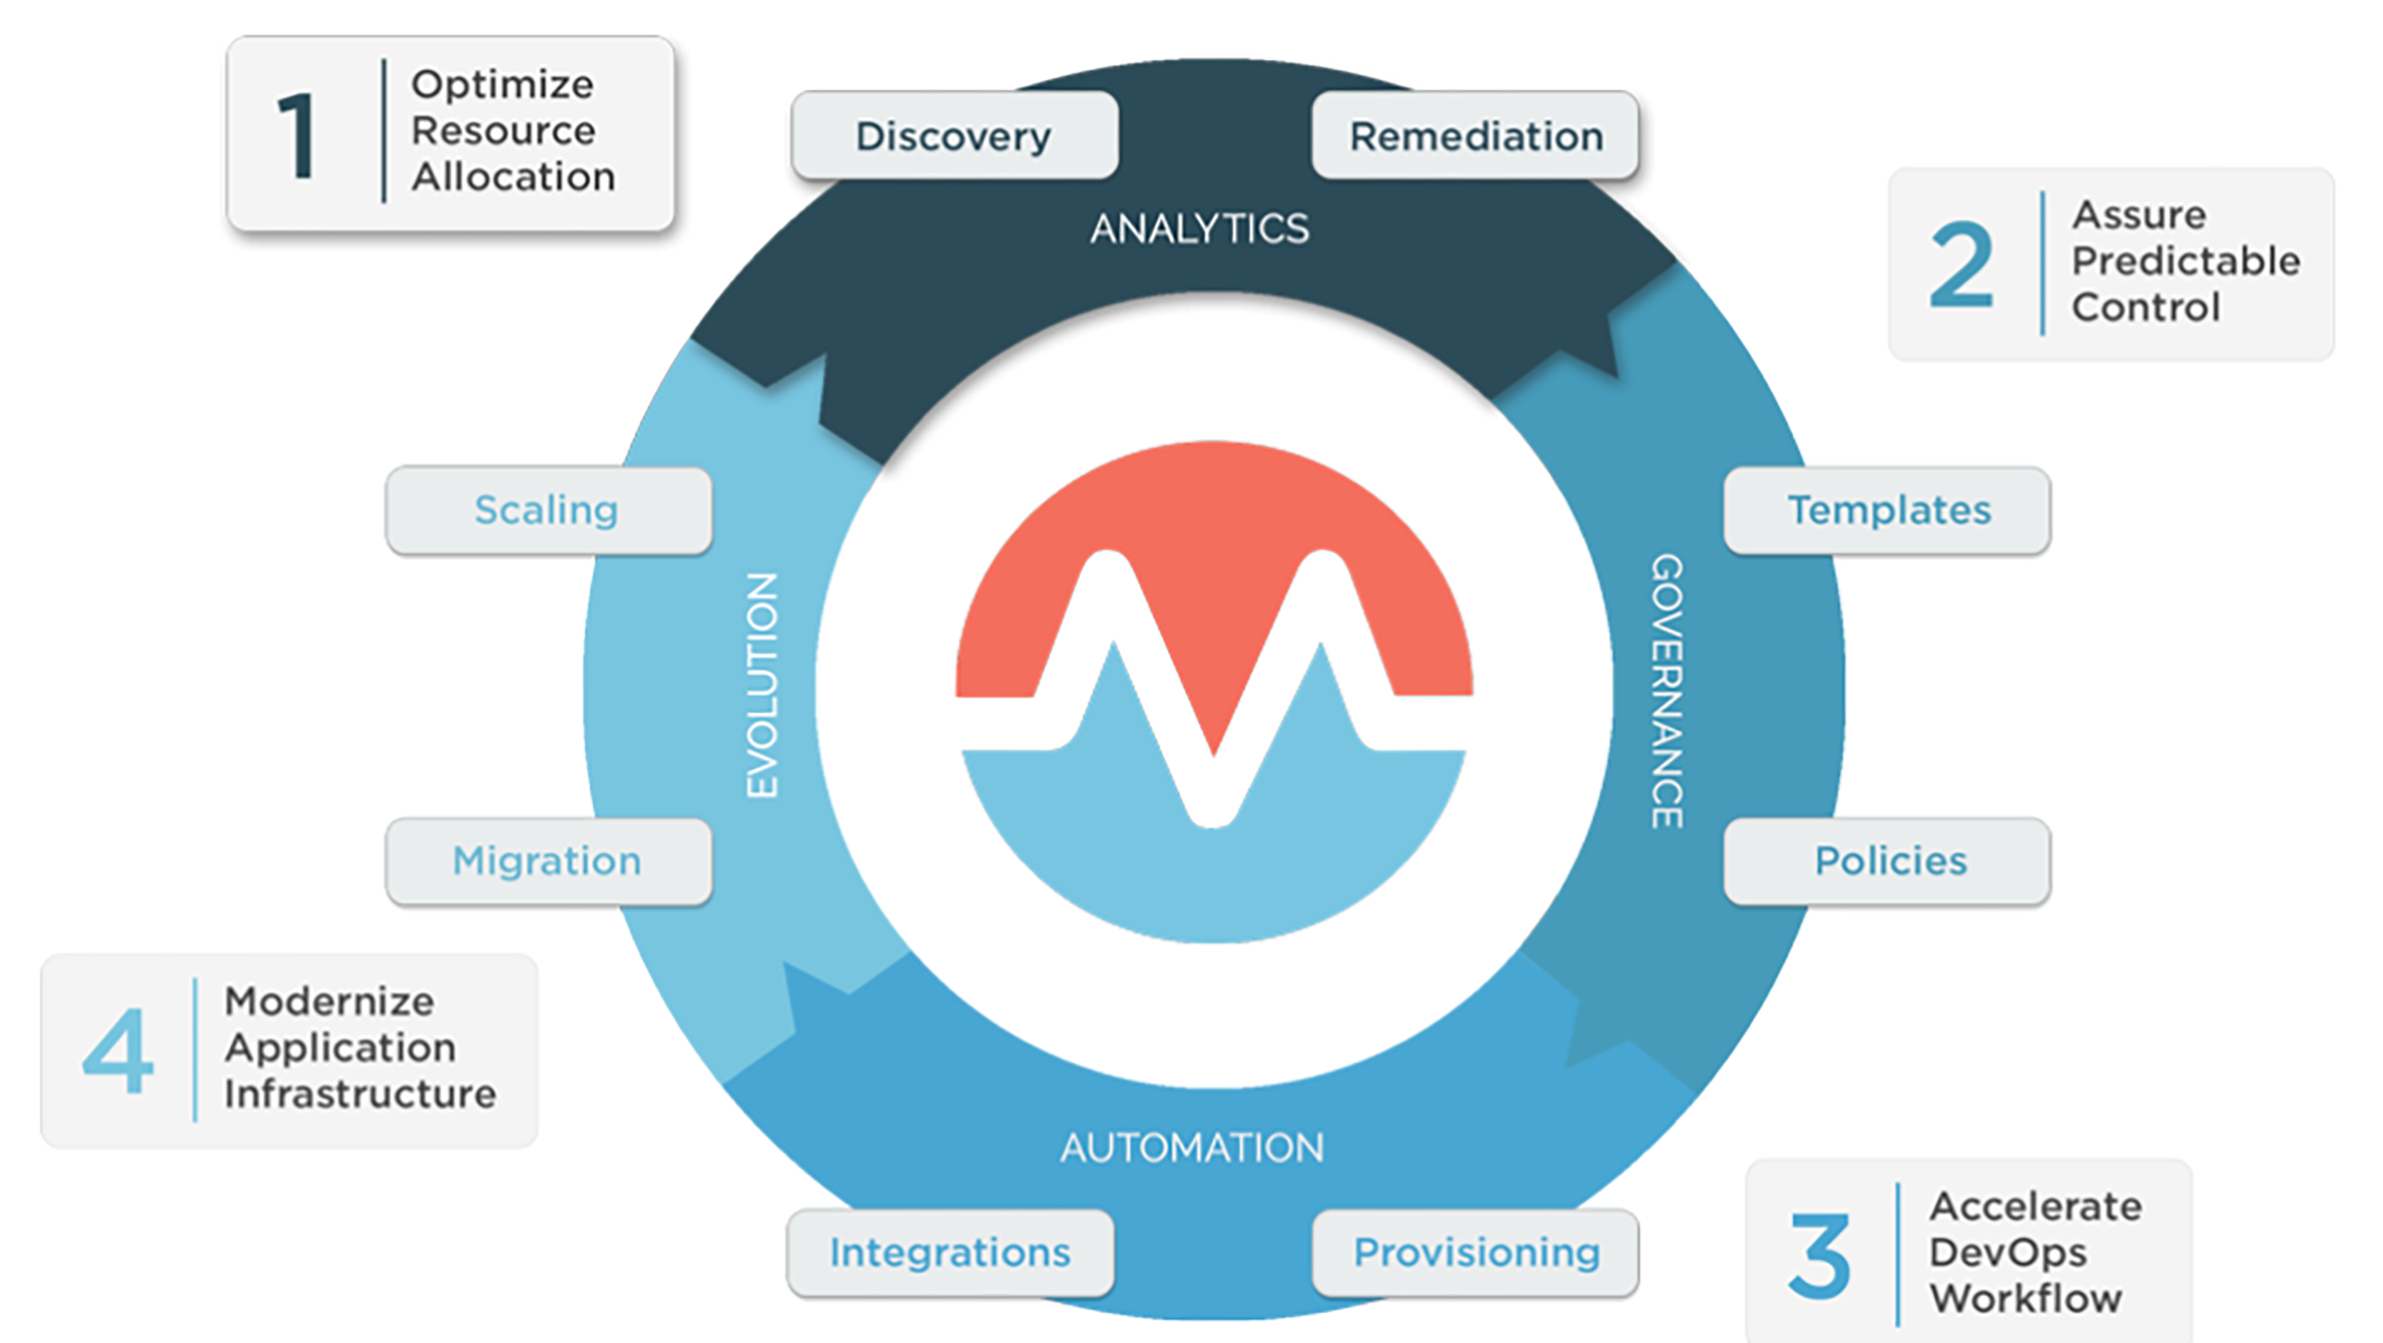
\includegraphics[width=\columnwidth]{../images/MorpheusSolutions.png}
	\caption{Morpheus Solutions~\cite{hid-sp18-416-www-morpheus-solutions}}
\label{fig:solutions}
\end{figure}


\subsection{Optimize Resource Allocation}

The problem addressed in this section is the high cost of allocating different 
resources and the wastage of resources. Morpheus helps with the provisioning of 
resources using the \textit{Analytics} product by means of \textit{Discovery} 
and \textit{Remediation}. Morpheus has the capability to gather data about the 
usage of resources and in many different environments. Morpheus is also capable 
of analyzing the gathered data and provide valuable information that can be 
used by its' users to choose the environment better suited for their 
application and choose remediation techniques to help avoid resource 
wastage~\cite{hid-sp18-416-www-morpheus-product-guide}. 

\subsection{Assure Predictable Control}

It is now easier than ever to gain access to cloud resources. This could cause 
employees to use tools that might not be permitted by their 
organization~\cite{hid-sp18-416-www-shadowit-wikipedia}. As an example 
consider an employee of the company using an on-line tool to decode secret keys 
necessary for a component. This allows a breach of secret keys used within a 
company and in wrong hands could do great harm to the company. These 
situations need to be avoided. Thus with the use of the \textit{Governance} 
product and its' elements such as \textit{Templates} and \textit{Policies}, 
Morpheus allows the ability for customers to use application templates and 
control access to environments by using different 
policies~\cite{hid-sp18-416-www-morpheus-product-guide}.  

\subsection{Accelerate DevOps Workflow}

It is inevitable that as organizations adapt to a cloud-first approach and 
start to deploy their codes in the cloud, the frequency of code deployments 
will increase. It will also get more complex as there are deployments spanning 
across multiple platforms and environments. This causes an increased workload 
for devlopers and DevOps professionals. With the \textit{Automation} product by 
means such as \textit{Integration} and \textit{Provisoning} Morpheus makes the 
workload of DevOps easier by introducing multiple tools that can be used 
easily. The manual process of deploying tools in environments is replaced by 
the support from Morpheus. Morpheus is capable of providing not only 
automation services but also services such as logging and 
monitoring~\cite{hid-sp18-416-www-morpheus-product-guide}.  

\subsection{Modernize Application Infrastructure}

Application infrastructure keeps changing over time, for example from 
traditional virtual machines to containers. With this continuous change in 
infrastructure, organizations find it hard to adapt their legacy applications 
to the ever changing infrastructure. But with Morpheus, it is possible to get a 
single view of the complete set of infrastructures and adopt different kinds of 
technologies. There is also support for easy migration from one technology to 
another as well as one technology version to another and auto-scaling. Morpheus 
provides this support with the use of the \textit{Architecture} product by 
means of \textit{Migration} and 
\textit{Scaling}~\cite{hid-sp18-416-www-morpheus-product-guide}.

\section{Integrations}
\label{sec:integrations}

Morpheus has many cloud integration choices such as clouds, automation tools, 
identity management, load balancing, DNS, storage, IPAM, backups, monitoring, 
logs, discovery, ITSM, containers, and deployments as shown in 
Figure~\ref{fig:integrations}. Examples 
for each of the categories are listed 
below~\cite{hid-sp18-416-www-morpheus-integrations}. 

\begin{figure}[htb]
	\centering
	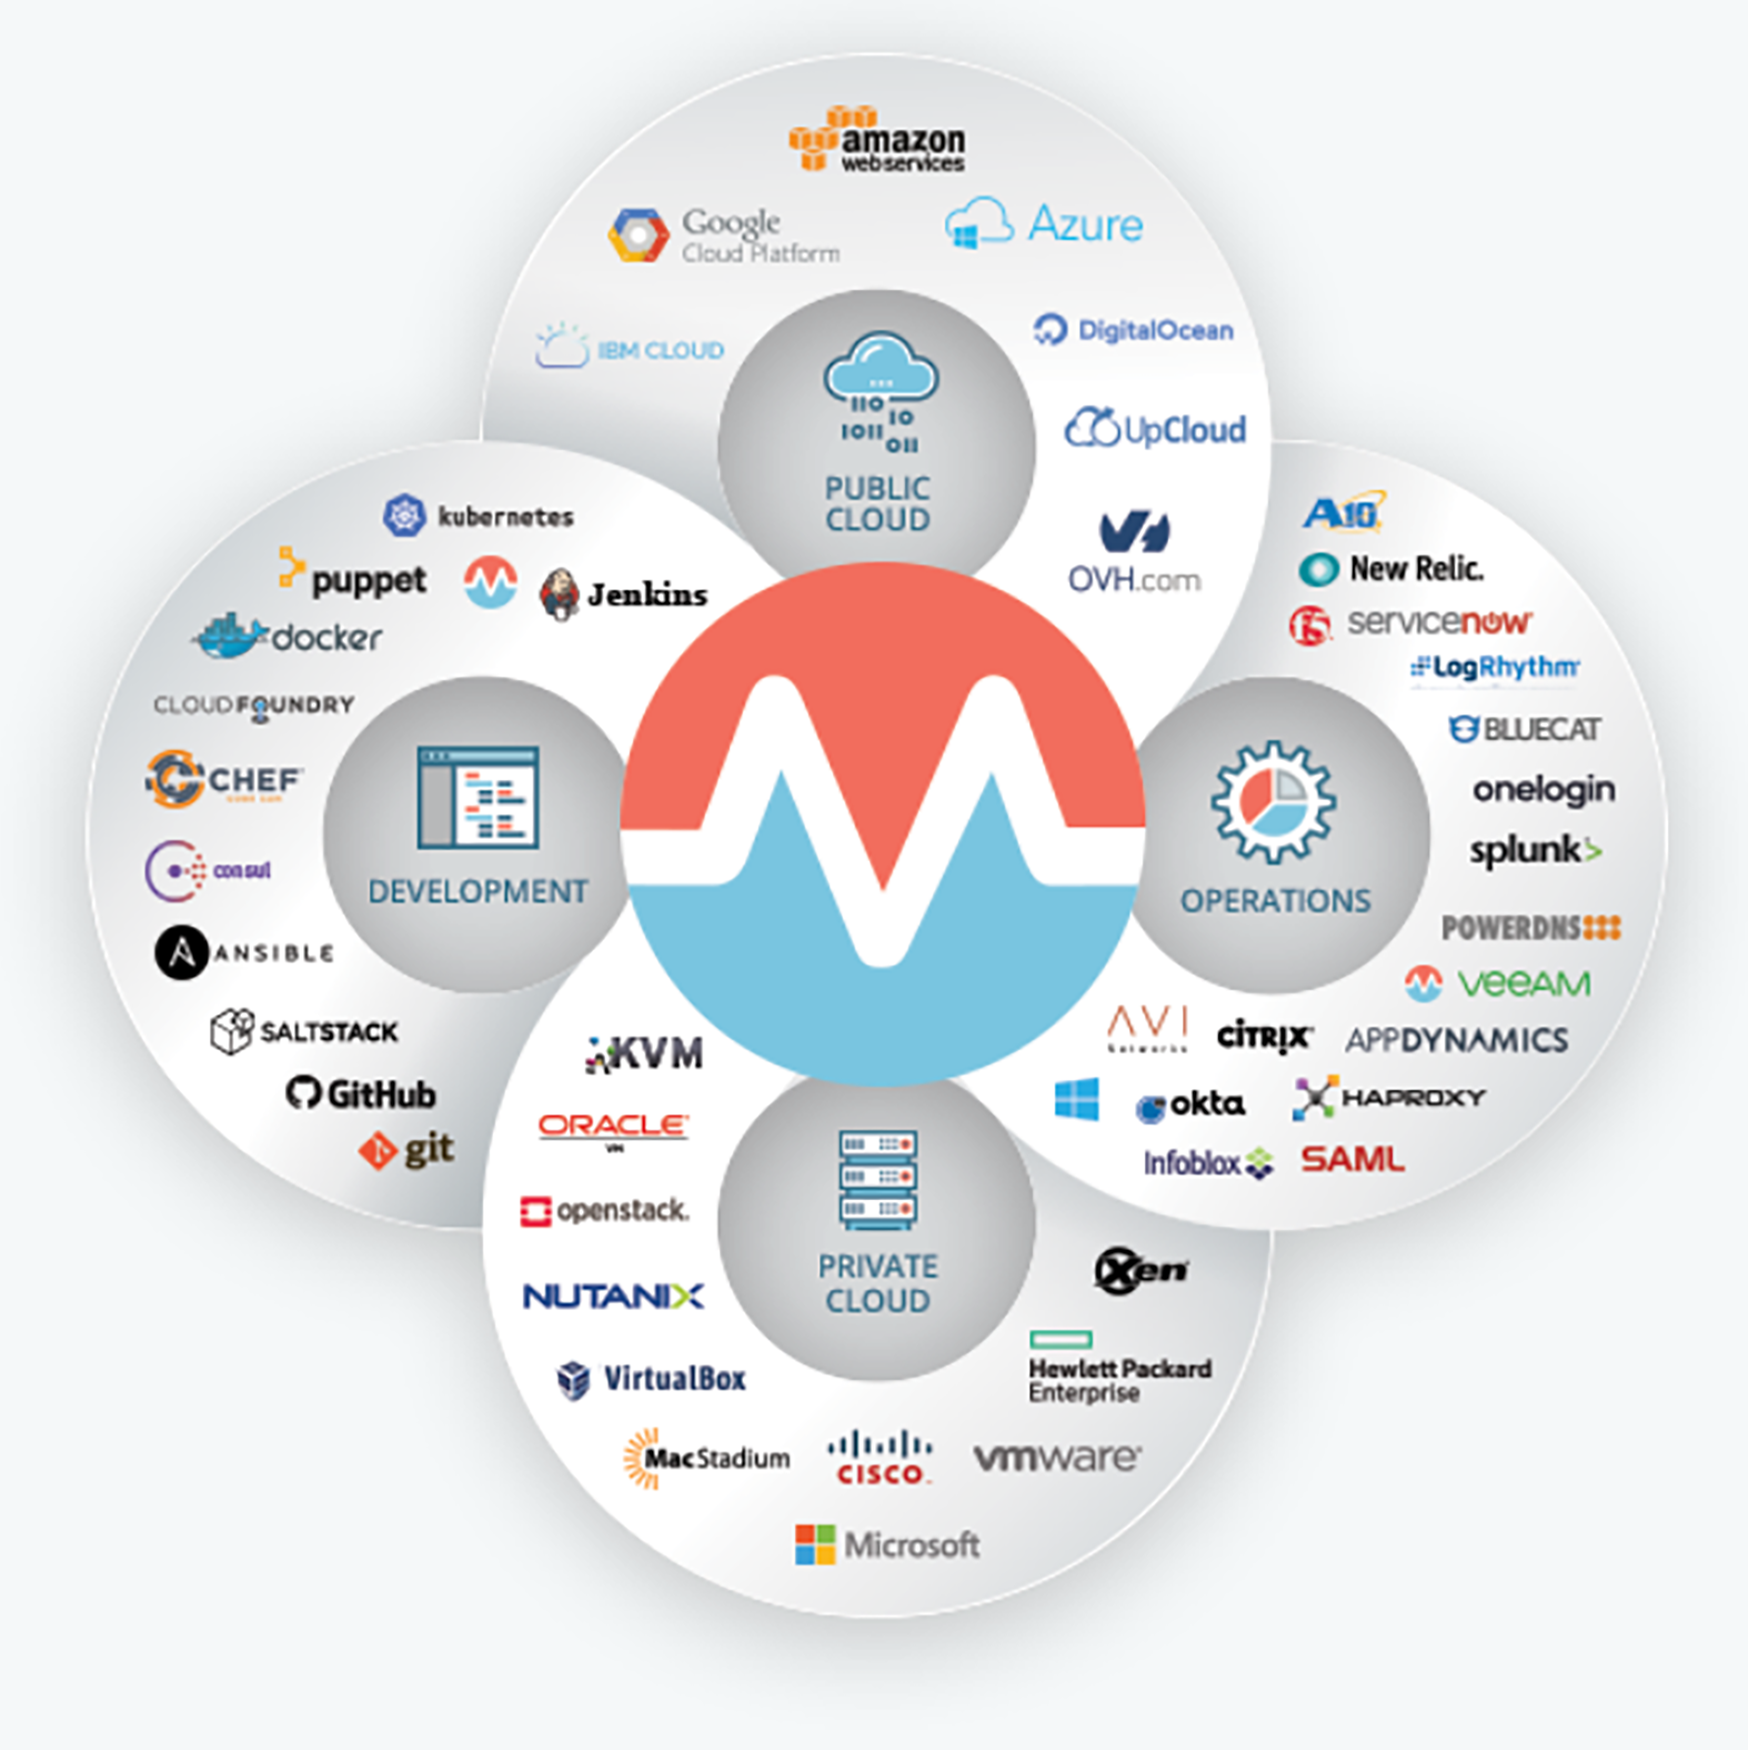
\includegraphics[width=\columnwidth]{../images/MorpheusIntegrations.png}
	\caption{Morpheus 
	Integrations~\cite{hid-sp18-416-www-morpheus-product-guide}}
\label{fig:integrations}
\end{figure}

\begin{itemize}
	\item \textbf{Public Clouds:} AWS, Azure, Softlayer, GCP, Digital 
	Ocean, vCloud Air
	\item \textbf{Private Clouds:} VMware, VMware ESXi, OpenStack, Hyper-V, 
	Azure Stack, Nutanix, Oracle VM, XenServer, VMWare Fusion, VirtualBox, 
	metacloud, KVM, Cisco UCS, MacStadium
	\item \textbf{Automation:} Puppet, Ansible, CHEF, SaltStack
	\item \textbf{Identity Management:} LDAP, okta, SAML, Microsoft Active 
	Directory, JumpCloud, OneLogin, Custom External, Custom API
	\item \textbf{Load Balancers:} F5, ACI, A10, Citrix, HAProxy, Amazon ALB, 
	Anazon ELB, Azure Load Balancer
	\item \textbf{DNS:} Microsoft DNS, Power DNS, Route 53
	\item \textbf{Storage:} Local storage, Amazon S3, OpenStack, Azure Storage, 
	Rackspace, CIFS, NFS, 3Par
	\item \textbf{IPAM:} IPAM internal, Infoblox, Bluecat
	\item \textbf{Backups:} Backups internal, Veeam, Commvault
	\item \textbf{Monitoring:} Morpheus Monitoring, App Dynamics, New Relic, 
	Service Now
	\item \textbf{Logs:} Morpheus, Syslog, Splunk, LogRhythm
	\item \textbf{Service Discovery:} Consul
	\item \textbf{ITSM:} ServiceNow
	\item \textbf{Containers:} Docker, Kubernetes, Docker Swarm, Nexus + Docker
	\item \textbf{Deployments:} Git, Jenkins  
\end{itemize}

\section{Customers}
\label{sec:customers}

The CIO of \textit{Spireon} states ``Morpheus has been a game changer for us. 
It has allowed for us to keep costs low and get our infrastructure up and 
running very quickly'', which provides us with essentially the vision of 
Morpheus~\cite{hid-sp18-416-www-morpheus-silicon-review}. Morpheus targets to 
bring its customers to the digital age by providing them with the heterogeneous 
platforms, deployments, storage, applications, and servers. In major cloud 
deployments the qualities that are lacking are the inability to easily 
integrate the legacy applications into cloud-first deployments, high cost due 
to the inefficiency of resource management and the inability to deploy faster.

Morpheus is being used by customers such as 
McDonald's~\cite{hid-sp18-416-www-mcdonalds}, 
BLACKROCK~\cite{hid-sp18-416-www-blackrock}, HSBC~\cite{hid-sp18-416-www-hsbc}, 
Spireon~\cite{hid-sp18-416-www-spireon}, ARRIS~\cite{hid-sp18-416-www-arris}, 
WGU~\cite{hid-sp18-416-www-wgu}, 
AstraZeneca~\cite{hid-sp18-416-www-astrazeneca}, 
Quicken Loans~\cite{hid-sp18-416-www-quickenloans} and 
GBG~\cite{hid-sp18-416-www-gbg}. The customers range from fast food chains, 
investment management corporations, banks, biopharmaceutical companies, 
mortgage lenders, private on-line universities to identity data intelligence 
providers. The list of customers is proof of the vast impact Morpheus has made 
on many different domains. It is evident that many companies tend to move from 
typical legacy applications to cloud-first applications. The requirement of 
each company might differ, but the agility provided by Morpheus is key to the 
success~\cite{hid-sp18-416-www-morpheus-customers}. 

\section{Pricing}
\label{sec:pricing}

Morpheus is a commercial tool which provides its services to the lowest quote 
of 25,000 U.S. Dollars. At the lowest \textit{Essentials} package users are 
able to obtain the basic services expected from a cloud orchestration tool 
which are the service platforms such as virtual machines, bare metal servers or 
containers across all clouds and its provisioning and orchestration. The more 
advanced packages of Morpheus are \textit{Pro} and \textit{Enterprise} which 
both contain capabilities to provision resources based on the requirement and 
can be provided automatically along with the features provided in the lower 
tier. Another feature common to both packages is the ability to integrate with 
the customer deployed third-party tools for various activities such as logging, 
backup, code repositories and many more. The \textit{Enterprise} package is the 
package offering the most important features such as multi-tenancy and 
customizable private themes and logos~\cite{hid-sp18-416-www-morpheus-pricing}. 

\section{Summary}
\label{sec:summary}

In conclusion, this technology paper provides an overview of the Multi-cloud 
Orchestration tool Morpheus. Morpheus provides four core products, namely 
analytics, governance, automation, and evolution. The core vision of Morpheus 
is to solve many problems faced by organizations with the use of different 
clouds, platforms and database types. Morpheus also aims to make the transition 
from the legacy systems to the cloud-first applications smoother.  
 
Morpheus is a tool solely focused on cloud orchestration and management. 
Currently, there are many companies who use Morpheus as such a tool. 
Examples of some of the organizations are McDoanlds', HSBC, BLACKROCK, Spireon, 
and WGU. These organizations belong to different domains showing the 
applicability of cloud across many domains and the existence of challenges 
that comes with it. Morpheus can be viewed as a core tool for companies that 
would like to make the digital transformation and increase the efficiency of 
companies by allowing 100x faster deployments and 30\% cost reductions.  

\begin{acks}

  The authors would like to thank Dr.~Gregor~von~Laszewski for his
  support and suggestions to write this paper.

\end{acks}

\bibliographystyle{ACM-Reference-Format}
\bibliography{report} 

